\documentclass[11pt]{article}
\usepackage[margin=1.05in]{geometry}
\usepackage{amsmath,amssymb,amsthm,mathtools}
\usepackage{booktabs}
\usepackage{tikz}
\usetikzlibrary{decorations.pathmorphing,patterns,arrows.meta}
\usepackage[colorlinks=true,linkcolor=blue!50!black,citecolor=blue!50!black,urlcolor=blue!50!black]{hyperref}

\newtheorem{theorem}{Theorem}
\newtheorem{proposition}[theorem]{Proposition}
\newtheorem{lemma}[theorem]{Lemma}
\newtheorem{corollary}[theorem]{Corollary}
\theoremstyle{definition}
\newtheorem{definition}[theorem]{Definition}
\theoremstyle{remark}
\newtheorem{remark}[theorem]{Remark}

\newcommand{\HH}{\mathbb{H}}
\newcommand{\CC}{\mathbb{C}}
\newcommand{\RR}{\mathbb{R}}
\newcommand{\ZZ}{\mathbb{Z}}
\newcommand{\SLZ}{\mathrm{SL}_2(\ZZ)}
\newcommand{\Li}{\mathrm{Li}}
\newcommand{\e}{\mathrm{e}}

\title{The branch choice in $L$-functions of weakly holomorphic\\ modular forms,
read as a choice of $(1-T)^{-1}$}
\author{Working note, project ``Hecke and MFs with poles'' (drafted with Claude)}
\date{24 September 2026}

\begin{document}
\maketitle

\begin{abstract}
For $f\in M^!_k$ with a pole at the cusp, the $L$-series of Bringmann--Fricke--Kent contains,
for each polar Fourier mode $c(-m)q^{-m}$, incomplete gamma functions $\Gamma(s,z)$ at the
negative real argument $z=-2\pi m$. That point lies on the branch cut, so the series
implicitly requires a choice of side. Diamantis--Lee--Raji--Rolen fix the principal
branch. This note makes the choice explicit and says what it means. The finite-contour
$L$-integral of the project draft uses a Hurwitz $T$-kernel, which solves a shift-difference
equation, i.e.\ inverts $1-T$. The two one-sided inversions $h_\pm$ unfold into horizontal
Mellin rays inside $\HH$, one running to the right and one to the left. They reproduce
exactly the two sides of the cut, and $h_+$ is the principal branch. Their difference is a
residue at $q=0$:
\[
L^*_+(f,s)-L^*_-(f,s)
=-2\pi i\Big[\tfrac{D(f,s)}{(2\pi)^s\Gamma(1-s)}
+i^k\tfrac{D(f,k-s)}{(2\pi)^{k-s}\Gamma(1-k+s)}\Big],
\qquad D(f,s)=\sum_{m\ge1}c_f(-m)m^{-s}.
\]
This is \emph{not} a new term. It is the sum of the per-mode jumps across the cut. The two
sides are complex conjugates at real $s$, so their mean is real (a principal value). The
note contributes three things: an explicit account of a choice that is usually made
silently; a dictionary identifying the side of the cut of $\Gamma(s,\cdot)$ with a one-sided
coboundary inversion of $1-T$ and with the direction of a horizontal Mellin ray; and
consequences of that dictionary. The choice is invisible on $M_k$ and at the critical
integers. The functional equation forces the same side at both cusps. The
principal-branch values are not real on the real axis. Every step takes place inside $\HH$,
on individual Fourier modes, or at the isolated point $q=0$; $f$ is never continued across
the real axis.
\end{abstract}

\section{Framing, and the natural-boundary concern}

\paragraph{What this note is, and is not.}
Passing from decaying Fourier modes ($n>0$) to growing ones ($n<0$) in the incomplete-gamma
representation is an analytic continuation in the argument of $\Gamma(s,\cdot)$. That
continuation lands on the cut, so it involves a choice, and that choice is the entire
content of the ambiguity studied here. We do not claim a new term or a new invariant. We
claim a precise account of the choice (Theorem~\ref{thm:main}, Proposition~\ref{prop:jump}) and an
identification of it with the coboundary freedom in inverting $1-T$. That second
freedom is the one that already appears on the cocycle side when period polynomials are
built from the same kernel at integer $s$.

\paragraph{The natural-boundary concern.}

A modular form lives on $\HH$. The real line is a natural boundary: every rational
point is a cusp, and for $f$ with a pole at $i\infty$ the modular transformation law
makes $f$ grow exponentially along every geodesic ending at a rational. So a phrase
like ``rotate the Mellin contour of $f$ into the lower half-plane'' has no meaning.
In an earlier informal explanation we used exactly that phrase. It is only correct
for \emph{individual Fourier modes} $q^n=\e^{2\pi i n\tau}$, which are entire in $\tau$.
This note replaces that heuristic with statements that stay inside the domain of $f$:
\begin{enumerate}
\item The two kernels unfold into two horizontal Mellin rays inside $\HH$
  (Lemma~\ref{lem:unfold}).
\item For $f$ with a pole at the cusp, horizontal is the only admissible direction for
  a ray, so there are exactly two choices (Lemma~\ref{lem:directions}).
\item No deformation inside $\HH$ connects the two rays. Going over the top is
  blocked by the pole at $q=0$, and going underneath is blocked by the natural
  boundary. The obstruction is measured \emph{exactly} by the residue at $q=0$
  (Theorem~\ref{thm:main}). In the $q$-coordinate, the cusp $i\infty$ is an isolated
  singular point, while every other cusp lies on the circle $|q|=1$.
\end{enumerate}
The lower half-plane and the Stokes-type branch jump of $\Gamma(s,z)$ return only in
Section~\ref{sec:modes}, as a computation carried out on finitely many entire
Fourier modes.

\section{Setup}

Let $k$ be even and $f\in M^!_k$ (no interior poles; see Remark~\ref{rem:interior}),
with $f(\tau)=\sum_{n\ge -M}c(n)q^n$. Let $S=\left(\begin{smallmatrix}0&-1\\1&0\end{smallmatrix}\right)$,
$T=\left(\begin{smallmatrix}1&1\\0&1\end{smallmatrix}\right)$. Powers $\tau^w$ use the principal
branch on $\CC\setminus(-\infty,0]\supset\HH$. For $\tau\in\HH$ we have
$\arg(-1/\tau)=\pi-\arg\tau$. Hence, with the weight $2-k$ action
$(g|_{2-k}\gamma)(\tau)=(c\tau+d)^{k-2}g(\gamma\tau)$ and $\varphi_s(\tau)=\tau^{s-1}$,
\begin{equation}\label{eq:phiS}
\varphi_s|_{2-k}S=\e^{i\pi(s-1)}\,\tau^{k-1-s}\qquad\text{exactly on }\HH .
\end{equation}

\begin{definition}[One-sided inversions of $1-T$]
For $\tau\in\HH$ and $\operatorname{Re}w<-1$ put
\[
h_+[w](\tau)=\sum_{n\ge1}(\tau+n)^w=\zeta(-w,\tau+1),\qquad
h_-[w](\tau)=-\sum_{n\le0}(\tau+n)^w=-\e^{i\pi w}\zeta(-w,-\tau),
\]
and continue meromorphically in $w$. (In the closed form of $h_-$ the Hurwitz argument
$-\tau$ lies in the lower half-plane. This is an evaluation of the elementary function
$\zeta(-w,\cdot)$ only; $f$ is never evaluated off $\HH$ anywhere in this note, except for
individual Fourier modes in Section~\ref{sec:modes}.) Both satisfy
$h[w](\tau)-h[w](\tau-1)=-\tau^w$. Define
$K_\pm(\tau,s)=h_\pm[s-1](\tau)-\e^{i\pi(s-1)}h_\pm[k-1-s](\tau)$, so that
$K_\pm(\tau)-K_\pm(\tau-1)=-(\varphi_s|_{2-k}(1-S))(\tau)$. The kernel $K_+$ is the Hurwitz
$T$-kernel $\widetilde k_T$ of the draft.
\end{definition}

\begin{definition}[Finite-contour $L$-integral]
For $\tau_0\in\HH$, $\gamma^S:-1/\tau_0\to\tau_0$ and $\gamma^T:\tau_0-1\to\tau_0$,
\[
L^*_\pm(f,s)=\e^{-\pi i s/2}\Big(\int_{\gamma^S}f(\tau)\tau^{s-1}d\tau
+\int_{\gamma^T}f(\tau)K_\pm(\tau,s)\,d\tau\Big).
\]
\end{definition}

Differentiating in $\tau_0$ with $f(-1/\tau)=\tau^kf(\tau)$ and \eqref{eq:phiS}, the
$S$-segment contributes $f(\tau_0)(\varphi_s|(1-S))(\tau_0)$ and the $T$-segment
contributes $f(\tau_0)(K(\tau_0)-K(\tau_0-1))$. These cancel for \emph{any} solution
$K$ of the shift equation. So basepoint independence cannot select a kernel. The
solutions form $K_++\{\text{1-periodic functions}\}$.

\section{Unfolding: the kernels are horizontal Mellin rays}

\begin{lemma}\label{lem:unfold}
Let $\gamma^T$ be the horizontal segment at height $y_0=\operatorname{Im}\tau_0$ and
$\operatorname{Re}w<-1$. Then
\[
\int_{\tau_0-1}^{\tau_0}f\,h_+[w]\,d\tau=\int_{0}^{\infty}f(\tau_0+t)\,(\tau_0+t)^w\,dt,\qquad
\int_{\tau_0-1}^{\tau_0}f\,h_-[w]\,d\tau=-\int_{-\infty}^{0}f(\tau_0+t)\,(\tau_0+t)^w\,dt,
\]
with $t\in\RR$. Both right-hand integrals therefore run along the horizontal line
$\operatorname{Im}\tau=y_0>0$, to the right and to the left respectively, and converge
absolutely. Along the left ray $\arg\tau\to\pi$ but stays below $\pi$, so $\tau^w$ never
meets its cut. The ``endpoint at infinity'' is the cusp $\infty\in\mathbb{P}^1$, approached at fixed height.
\end{lemma}
\begin{proof}
On the line, $f$ is continuous and $1$-periodic, hence bounded. Since $|\tau^w|\le C|\tau|^{\operatorname{Re}w}$,
the sum $\sum_n$ converges uniformly on the segment, and we may exchange it with the
integral. Periodicity gives
$\int_{\tau_0-1}^{\tau_0}f(\tau)(\tau+n)^w\,d\tau=\int_{\tau_0-1+n}^{\tau_0+n}f(u)u^w\,du$.
Summing over $n\ge1$ tiles the right ray; summing over $n\le0$ tiles the left ray.
\end{proof}

So for $\operatorname{Re}s<0$ the first half of $K_+$ is the Mellin integral of $f$ along
the horizontal ray from $\tau_0$ to the right. The second half, valid for
$\operatorname{Re}s>k$, becomes the same kind of ray integral against $\tau^{k-1-s}$.
The substitution $u=-1/\tau$ turns it into a Mellin integral of $f\,u^{s-1}$ along the
$S$-image of the ray. That image is an arc of the horocycle $|u-\tfrac{i}{2y_0}|=\tfrac1{2y_0}$,
which approaches the cusp $0$ tangentially from the left, since
$u=-1/(t+iy_0)$ has $\operatorname{Re}u<0$.

Put together, and with each piece continued separately in $s$, $L^*_+$ is the Mellin
integral of $f$ along a path from the cusp $0$ to the cusp $\infty$. It follows the
classical route, but enters and leaves both cusps \emph{horocyclically}, not along
the geodesic $i\RR_{>0}$ (Figure~\ref{fig:paths}). $L^*_-$ is its mirror image under
$\tau\mapsto-\bar\tau$.

\begin{figure}[t]
\centering
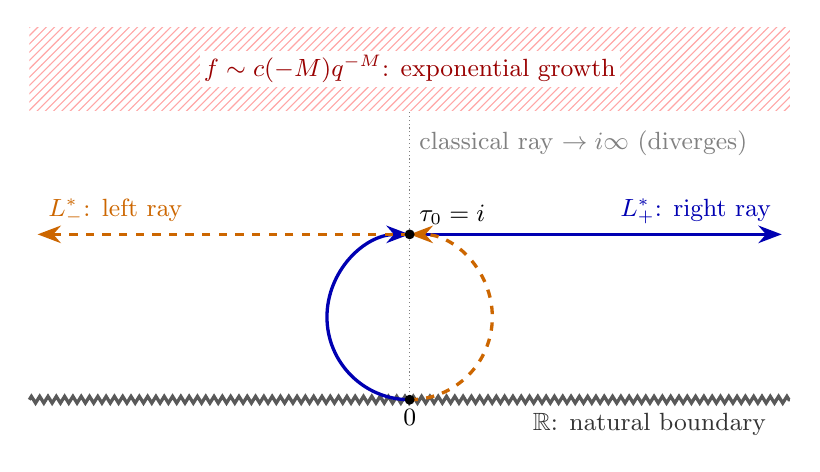
\begin{tikzpicture}[scale=2.1,>=Stealth]

  \fill[pattern=north east lines,pattern color=red!35] (-2.3,1.75) rectangle (2.3,2.25);
  \node[red!60!black,fill=white,inner sep=1.5pt] at (0,2.0) {\small $f\sim c(-M)q^{-M}$: exponential growth};

  \draw[very thick,decorate,decoration={zigzag,segment length=3pt,amplitude=1.2pt},gray!70!black] (-2.3,0)--(2.3,0);
  \node[gray!40!black,below] at (1.45,-0.02) {\small $\RR$: natural boundary};

  \draw[densely dotted,gray] (0,0)--(0,1.75);
  \node[gray,right] at (0,1.55) {\small classical ray $\to i\infty$ (diverges)};

  \draw[blue!70!black,very thick,->] (0,1)--(2.25,1) node[above left]{\small $L^*_+$: right ray};
  \draw[blue!70!black,very thick,->] (0,0) arc[start angle=-90,end angle=-270,radius=0.5];

  \draw[orange!80!black,very thick,dashed,->] (0,1)--(-2.25,1) node[above right]{\small $L^*_-$: left ray};
  \draw[orange!80!black,very thick,dashed,->] (0,0) arc[start angle=-90,end angle=90,radius=0.5];
  \fill (0,1) circle (0.03) node[above right]{\small $\tau_0=i$};
  \fill (0,0) circle (0.03) node[below]{\small $0$};
\end{tikzpicture}
\caption{The two unfolded Mellin paths for $\tau_0=i$ (where $\gamma^S$ degenerates).
Solid: $L^*_+$ enters the cusp $0$ along a horocycle from the left and leaves toward
$\infty$ horizontally to the right. Dashed: $L^*_-$, the mirror image. Neither path can
be deformed into the other: the region above (the cusp $i\infty$) and the real axis
below are both forbidden.}
\label{fig:paths}
\end{figure}

\section{Why exactly two: admissible directions and the two walls}

\begin{lemma}\label{lem:directions}
Let $M\ge1$ and $c(-M)\ne0$. For the ray $\rho_\theta(t)=\tau_0+t\e^{i\theta}$, $t\ge0$:
\begin{enumerate}
\item[(a)] if $0<\theta<\pi$, then $\int_{\rho_\theta}f(\tau)\tau^w\,d\tau$ diverges for every $w\in\CC$;
\item[(b)] if $\theta\in\{0,\pi\}$, it converges absolutely for $\operatorname{Re}w<-1$;
\item[(c)] if $\pi<\theta<2\pi$, the ray reaches $\RR$ at finite $t$, where $f$ is not defined.
\end{enumerate}
\end{lemma}
\begin{proof}
(a) As $\operatorname{Im}\tau\to\infty$ uniformly in $\operatorname{Re}\tau$, we have $f(\tau)=c(-M)q^{-M}(1+O(\e^{-2\pi\operatorname{Im}\tau}))$.
Along $\rho_\theta$, $|q^{-M}|=\e^{2\pi M(y_0+t\sin\theta)}$ grows exponentially, while $|\tau^w|$ changes only
polynomially. The partial integrals therefore grow exponentially. (b) is Lemma~\ref{lem:unfold}.
(c) holds because the ray leaves $\HH$.
\end{proof}

\paragraph{The natural boundary.}
For $\gamma=\left(\begin{smallmatrix}a&b\\c&d\end{smallmatrix}\right)\in\SLZ$ with $c\neq 0$,
$f(\gamma\tau)=(c\tau+d)^kf(\tau)$. As $\tau\to i\infty$, $\gamma\tau$ tends to $a/c$ along a
geodesic, and $|f(\gamma\tau)|$ grows like $\e^{2\pi M\operatorname{Im}\tau}$. So $f$ blows up
exponentially at a dense set of real points and has no holomorphic continuation across
any real interval. The following bookkeeping records what may legitimately be done with
each object.

\begin{center}\small
\begin{tabular}{@{}p{0.2\textwidth}p{0.36\textwidth}p{0.36\textwidth}@{}}
\toprule
object & domain of holomorphy & allowed operations\\\midrule
$f$ & $\HH$ (in $q$: $0<|q|<1$, pole of order $M$ at $0$) & deform contours inside $\HH$ only\\
single mode $q^n$ & all of $\CC$ & deform anywhere (mind the cut of $\tau^w$)\\
$\tau^w$, $h_\pm[w]$ & $\CC$ minus a cut & continue freely, but never pair with $f$ off $\HH$\\
$F(q)=f(\tau)$ & $0<|q|<1$; $|q|=1$ is a natural boundary & residues at $q=0$\\
\bottomrule
\end{tabular}
\end{center}

\paragraph{Consequence.}
For a cusp form ($M=0$, $c(0)=0$), $f$ decays at $i\infty$, and every ray with
$\theta\in[0,\pi]$ gives the same value. Deforming through the region near the cusp is
legitimate, because the arcs at infinity vanish. For $M\ge1$ that region is forbidden,
and the real axis is forbidden for any $f$. The two admissible rays are separated above
by the cusp and below by the natural boundary. Their difference is therefore a
well-defined obstruction and need not vanish. We compute it next.

\section{The difference is a residue at the cusp}

\begin{lemma}[Lipschitz]\label{lem:lip}
For $\tau\in\HH$ and $\operatorname{Re}w<-1$,
\[
\Lambda_w(\tau):=\sum_{n\in\ZZ}(\tau+n)^w=\frac{(-2\pi i)^{-w}}{\Gamma(-w)}\sum_{r\ge1}r^{-w-1}q^r .
\]
In particular
\[
h_+[s-1]-h_-[s-1]=\Lambda_{s-1}=\frac{(-2\pi i)^{1-s}}{\Gamma(1-s)}\Li_s(q),
\]
and this identity continues meromorphically in $s$.
\end{lemma}

$\Lambda_w$ is $1$-periodic, so it descends to the $q$-disc, where it is holomorphic and
vanishes at $q=0$. It is precisely a ``periodic correction'' of the kernel.

\begin{theorem}\label{thm:main}
For $f\in M^!_k$ and all $s$ (as an identity of meromorphic functions),
\[
L^*_+(f,s)-L^*_-(f,s)=-2\pi i\left[\frac{D(f,s)}{(2\pi)^s\,\Gamma(1-s)}
+i^k\,\frac{D(f,k-s)}{(2\pi)^{k-s}\,\Gamma(1-k+s)}\right],\quad
D(f,s)=\sum_{m=1}^{M}\frac{c(-m)}{m^{s}}.
\]
\end{theorem}
\begin{proof}
First, $L^*_+-L^*_-=\e^{-\pi is/2}\int_{\gamma^T}f\,[\Lambda_{s-1}-\e^{i\pi(s-1)}\Lambda_{k-1-s}]\,d\tau$.
By Lemma~\ref{lem:unfold}, $\int_{\gamma^T}f\Lambda_w$ equals the Mellin integral of $f$ over
the \emph{full} horizontal line: right ray minus left ray. To evaluate it, put
$q=\e^{2\pi i\tau}$. The segment becomes the circle $|q|=\e^{-2\pi y_0}$, traversed once
counter-clockwise, and $d\tau=dq/(2\pi i q)$. Then
\[
\int_{\tau_0-1}^{\tau_0}f\,\Lambda_w\,d\tau=\oint\frac{F(q)\Lambda_w(q)}{2\pi i\,q}\,dq
=\operatorname*{Res}_{q=0}\frac{F\Lambda_w}{q}
=\frac{(-2\pi i)^{-w}}{\Gamma(-w)}\sum_{m\ge1}c(-m)\,m^{-w-1}.
\]
The only singularity of $F\Lambda_w/q$ inside the circle is at $q=0$; the natural
boundary $|q|=1$ is never approached. Taking $w=s-1$ and $w=k-1-s$ and simplifying the
phases with \eqref{eq:phiS} gives the claim.
\end{proof}

\begin{corollary}\label{cor}
\begin{enumerate}
\item[(i)] $L^*_+=L^*_-$ on $M_k$. The constant term is unambiguous too, since $\Lambda_w$ has
no $q^0$ term.
\item[(ii)] $L^*_+=L^*_-$ at $s\in\{1,\dots,k-1\}$, because $1/\Gamma$ vanishes there. Periods and critical
values are canonical.
\item[(iii)] The two terms are the choices made at the two cusp ends of the path in
Figure~\ref{fig:paths}. The term $D(f,s)$ belongs to $\infty$, and the term $D(f,k-s)$ belongs to $0$. The
data at $0$ is the same principal part, transported by $S$. The functional equation
$L^*(s)=i^kL^*(k-s)$ holds for $K_+$, for $K_-$, and for every affine combination
$\lambda K_++(1-\lambda)K_-$. It \emph{fails} for the mixed kernel that uses $h_+$ in one half and
$h_-$ in the other (Table~\ref{tab:num}). So the functional equation forces the path to be
$S$-symmetric.
\end{enumerate}
\end{corollary}

\begin{remark}[What distinguishes ``right'' from ``left'']
In the $q$-disc, both horizontal rays wind infinitely often around the same circle and
never approach $q=0$. The distinction is invisible on $Y(1)$ and exists only on the
universal cover $\HH$. It arises because the Mellin weight $\tau^{s-1}$ is not
$T$-invariant, so one must decide in which direction to sum the $T$-orbit. The cusp of
$Y(1)$ has no ``sides''. The two sides are introduced by the non-invariant kernel, and
the residue at $q=0$ measures how much $f$ notices. Cohomologically, the ambiguity is
$\ker(1-T)$ on the kernel module. On the polynomial module $V_{k-2}$ (integer $s$) this
kernel consists of constants, which pair with $c(0)$ only. At non-integer $s$ it
contains $\Li_s(q)$, which pairs with the principal part.
\end{remark}

\section{The per-mode shadow: where the lower half-plane legitimately enters}\label{sec:modes}

The Bringmann--Fricke--Kent (BFK) formula at $\tau_0=i$ is
\[
L^*(f,s)=\sum_{n\ne0}c(n)\Big[\frac{\Gamma(s,2\pi n)}{(2\pi n)^s}+i^k\frac{\Gamma(k-s,2\pi n)}{(2\pi n)^{k-s}}\Big]-c(0)\Big(\frac1s+\frac{i^k}{k-s}\Big).
\]
It arises from integrating each Fourier mode separately. On the horizontal ray this is
rigorous: the Fourier series converges uniformly there, and by the bound in the proof of
Lemma~\ref{lem:unfold} we may exchange sum and integral. Each mode is now entire, so its own contour may
be rotated. For $n>0$ we rotate upward to $i\infty$, which reproduces the classical
incomplete gamma. The principal part has only finitely many modes $q^{-m}$, and each
decays in the \emph{lower} half-plane. So for these modes alone we rotate the horizontal
ray downward. This is legitimate for $q^{-m}\tau^w$ and meaningless for $f$. The right
ray, rotated clockwise, passes the branch point $\tau=0$ of $\tau^w$ on the right,
inside the cut plane. The left ray passes it on the left and lands on the other sheet.
The two results differ by a Hankel loop around $\tau=0$. The Hankel loop gives
$(-2\pi i)^{-w}m^{-w-1}/\Gamma(-w)$, which is the $q^m$ coefficient of $\Lambda_w$, in agreement
with Theorem~\ref{thm:main}.

Two remarks. First, the branch point of the kernel sits at $\tau=0$, which is itself a
cusp: the $S$-image of $i\infty$. The per-mode computation sees a branch point exactly
where $f$ has a natural-boundary point. The per-mode and global pictures agree only
because the sum over modes is taken \emph{on the horizontal ray, before any rotation}.
Summing rotated mode integrals over infinitely many modes and calling the result an
integral of $f$ in the lower half-plane would be meaningless. Second, in BFK's formula
the negative-$n$ terms are values of $z^{-s}\Gamma(s,z)$ on its cut $z<0$. Writing
$z^{-s}\Gamma(s,z)=\Gamma(s)z^{-s}-E$, with
\[
E(s,m):=\sum_{j\ge0}\frac{(2\pi m)^j}{j!\,(s+j)}\quad(z=-2\pi m),
\]
single-valued, only $\Gamma(s)z^{-s}$ depends on the branch. Its jump,
$\Gamma(s)(2\pi m)^{-s}(\e^{-i\pi s}-\e^{i\pi s})=-2\pi i(2\pi m)^{-s}/\Gamma(1-s)$, is exactly the term in
Theorem~\ref{thm:main}. This yields the following statement.

\begin{proposition}[Global difference $=$ summed per-mode jumps]\label{prop:jump}
Let $B_\pm(s,m)$ denote the polar-mode summand
$\frac{\Gamma(s,z)}{z^s}+i^k\frac{\Gamma(k-s,z)}{z^{k-s}}$ evaluated as the limit $z\to-2\pi m\pm i0$. Then
\[
L^*_+(f,s)-L^*_-(f,s)=\sum_{m\ge1}c(-m)\,\big[B_+(s,m)-B_-(s,m)\big],
\]
and $L^*_+$ equals the BFK series with every polar term taken from the upper side
($\arg z=+\pi$, the principal branch; this is the convention made explicit
in~\cite{DLRR}). $L^*_-$ takes every polar term from the lower side.
\end{proposition}
\begin{proof}
The jump of $z^{-a}\Gamma(a,z)$ across $z=-x$ is $-2\pi i\,x^{-a}/\Gamma(1-a)$. Summing this over
both halves and all polar modes reproduces the right-hand side of Theorem~\ref{thm:main}.
\end{proof}
This was checked independently of the closed-form jump. mpmath's own continuation of
$\Gamma(s,z)$ at $z=-2\pi m\pm10^{-30}i$ reproduces the kernel difference to $10^{-26}$ or better
(Table~\ref{tab:num}). The global Dirichlet-polynomial formula and the per-mode branch
picture are therefore the same ambiguity, seen at two scales. The link between them is
the Lipschitz formula. This is a computed identity, not something visible from the
shape of the formula.

\begin{remark}[The branch choice is a special case of a larger freedom]
The shift-difference equation allows any $1$-periodic correction $p(\tau,s)$ of the kernel. If $p$
is holomorphic at $q=0$, with $p=\sum_{n\ge0}p_n(s)q^n$, then $L^*$ changes by
$\e^{-\pi is/2}\sum_{m\ge0}c(-m)p_m(s)$. For instance, $p=q$ shifts $L^*$ by $\e^{-\pi is/2}c(-1)$,
which is not a branch effect of anything. The functional equation only requires
$\e^{-\pi is/2}p_m(s)$ to be symmetric under $s\leftrightarrow k-s$, which still leaves infinitely many
choices. The branch choice is the one-parameter subfamily obtained by inverting $1-T$ as a
one-sided sum over a $T$-orbit of $\tau^{s-1}$, together with affine combinations of the
two. Any principle that singles out these one-sided sums is extra input; it does not
follow from basepoint independence or from the functional equation.
\end{remark}

\paragraph{Branch-explicit formula.}
Averaging the two kernels gives, with $n=-m<0$,
\begin{multline*}
L^*_{\rm sym}(f,s)=\sum_{n>0}c(n)\Big[\tfrac{\Gamma(s,2\pi n)}{(2\pi n)^s}+i^k\tfrac{\Gamma(k-s,2\pi n)}{(2\pi n)^{k-s}}\Big]
-c(0)\Big(\tfrac1s+\tfrac{i^k}{k-s}\Big)\\
+\sum_{m\ge1}c(-m)\Big[\cos(\pi s)\big(\Gamma(s)(2\pi m)^{-s}+i^k\Gamma(k-s)(2\pi m)^{-(k-s)}\big)-E(s,m)-i^kE(k-s,m)\Big],
\end{multline*}
and $L^*_\pm=L^*_{\rm sym}\mp i\pi\big[\tfrac{D(f,s)}{(2\pi)^s\Gamma(1-s)}+i^k\tfrac{D(f,k-s)}{(2\pi)^{k-s}\Gamma(1-k+s)}\big]$.

\section{Reality: generic behaviour of a cut, and what it costs}

For real $s$ and real $x>0$, the two lateral values of $z^{-s}\Gamma(s,z)$ at $z=-x$ are complex
conjugates. This is the generic behaviour of a real-analytic function on its cut, and it has
nothing to do with modular forms. Their mean is real, and it is the natural principal value.
For $s=0$ this is literal: the two sides of $\Gamma(0,-x)$ are $-\mathrm{Ei}(x)\mp i\pi$, and
$\mathrm{Ei}(x)$ is defined by a Cauchy principal-value integral (checked at $x=2\pi$ to 40 digits).
So the reality of $L^*_{\rm sym}=\tfrac12(L^*_++L^*_-)$ is not a discovery. It is the statement that
one takes the principal value on the cut.

Geometrically, the map $\tau\mapsto-\bar\tau$ normalises $\SLZ$, conjugates $T$ to $T^{-1}$, and
exchanges the two horizontal rays. For $f$ with real coefficients, $f(-\bar\tau)=\overline{f(\tau)}$,
and $L^*_-(f,s)=\overline{L^*_+(f,s)}$ for real $s$ (checked numerically).

What does deserve to be recorded is the cost of the standard convention. When
$D(f,\cdot)\not\equiv0$, the principal-branch $L$-values (equivalently $L^*_+$) are \emph{not real} on the
real axis, even for $f$ with real coefficients. Anyone importing the intuition from $M_k$,
where real coefficients give real values at real $s$, would be misled. The imaginary part
is exactly half of the correction in Theorem~\ref{thm:main}. There is a formal resemblance to
lateral versus median Borel resummation: two admissible lateral directions, a forbidden
direction (here, toward the cusp), and an imaginary ambiguity. The mechanism here,
however, is a residue at a pole in the $q$-disc, not a Borel-plane singularity.

\section{Relation to the period theory of the project draft}\label{sec:periods}

The longer project draft attaches periods and quasi-periods to meromorphic forms. As
described there (the draft was not re-read for this note, so the details below are the
author's framing, not independently checked), two ambiguities arise:
\begin{enumerate}
\item[(a)] \emph{wall-crossing}: a contour crossing an interior pole shifts every special value
by a residue;
\item[(b)] \emph{subtraction}: the regularising subtraction is defined only modulo $S^!_k$,
a space of dimension $2\dim S_k$.
\end{enumerate}
For $\dim S_k=1$ ($k=12,16,18,20,22,26$), the periods of $\Delta_k=\Delta E_{k-12}$ and the
quasi-periods of $\hat\Delta_k=q^{-1}+O(q)$ span the $W^+\oplus W^-$ plane. The subtraction
coefficients are arbitrary complex numbers, so there is no lattice. Modulo subtraction,
the period vector is a smear that carries no information. The substantive question is
whether a \emph{canonical section} exists: a canonical rule for the subtraction. The choice
between $K_+$ and $K_-$ studied here is a small instance of the same question.

\begin{remark}[The branch choice is transverse to the subtraction smear; reasoned, unchecked]
By Corollary~\ref{cor}(ii), $L^*_+-L^*_-$ vanishes at every $s\in\{1,\dots,k-1\}$ (checked directly at
$s=3,6,9$ for $\Delta'$ and $g$). It therefore does not touch the $V_{k-2}$ period polynomial or
its $W^\pm$ coordinates. It is visible only at non-critical $s$, including $s=0$ and $s=k$,
where it is nonzero. This assumes the draft builds periods from $s=1,\dots,k-1$ only.
\end{remark}

\begin{remark}[Wall-crossing jumps are subtraction-invariant; reasoned, unchecked]
Subtracting a weakly holomorphic form adds no residues in $\HH$. Jumps across walls, and
hence differences of periods between homotopy classes of contours, are therefore
unaffected by the subtraction ambiguity, even though absolute periods are. If canonical
content survives the smear, relative periods are a natural place to look. A form with a
pole at a CM point ($i$ or $\rho$), where the Laurent data is algebraic, is the obvious test case.
\end{remark}

\section{Numerical checks}

All checks are reproduced by \texttt{verify\_kernel.py}, which reports 47/47 PASS with
\texttt{--slow}. They use \texttt{mpmath} at 30 digits and $\tau_0=i$. The test forms are
$\Delta'=\frac{E_6^2E_4^3}{\Delta}+\frac{5541}{16}E_4^3-\frac{1317}{16}E_6^2=q^{-1}+47709536q^2+\cdots$
(Brown~\cite{Brown}), and
$g=j\Delta'-744\Delta'=q^{-2}+196884+69203296q+\cdots$, so that $D(g,s)=2^{-s}$ tests the $m$-dependence.

\begin{table}[h]
\centering\footnotesize
\begin{tabular}{@{}lll@{}}
\toprule
check & form, $s$ & result\\\midrule
Lipschitz, Lemma~\ref{lem:lip} & pointwise, 3 values of $s$ & error $\le 4\cdot10^{-31}$\\
$L^*=\Lambda(G_k,s)$ on $M_k$ & $G_4,G_{12}$ & error $\le10^{-33}$\\
Theorem~\ref{thm:main} & $\Delta'$; $s=3.3,\ 5+1.5i,\ 0.37$ & error $\le 8\cdot10^{-31}$\\
Theorem~\ref{thm:main} & $g$; same $s$ & error $\le 2\cdot10^{-26}$\\
Corollary~\ref{cor}(ii), closed form & $\Delta'$, $g$; $s=1,\dots,11$ & exactly $0$\\
Corollary~\ref{cor}(ii), direct & $\Delta'$, $g$; $s=3,6,9$ & $|L^*_+-L^*_-|\le2\cdot10^{-31}$\\
correction at $s\to0$ & $\Delta'$ & $-2\pi i$ (nonzero)\\
Prop.~\ref{prop:jump} (mpmath limits $z\to-2\pi m\pm i0$) & $\Delta'$; $s=3.3,\,5+1.5i,\,0.37$ & error $\le2\cdot10^{-28}$\\
Prop.~\ref{prop:jump}, wrong side (control) & same & off by $0.012$, $0.17$, $4.4$\\
Prop.~\ref{prop:jump} & $g$; same $s$ & error $\le7\cdot10^{-26}$\\
$L^*_+$ vs BFK principal branch & $\Delta'$; $s=3.3,\ 5+1.5i$ & error $\le 2\cdot10^{-28}$\\
$L^*_-=\overline{L^*_+}$, real $s$ & $\Delta'$, $g$; $s=3.3,\,0.37$ & error $\le10^{-25}$\\
mean of sides of $\Gamma(0,-2\pi)$ vs $-\mathrm{Ei}(2\pi)$ & --- & equal to working precision\\
$L^*_{\rm sym}$ formula vs $\tfrac12(L^*_++L^*_-)$ & $\Delta'$; $s=3.3,\ 5+1.5i,\ -0.7$ & error $\le2\cdot10^{-28}$\\
functional equation, $K_\pm$ & $\Delta'$, $g$; $s=3.3,\ 5+1.5i$ & error $\le10^{-25}$\\
functional equation, mixed kernel & $\Delta'$ / $g$; same $s$ & fails by $0.014,\,0.38$ / $0.001,\,0.006$\\
Lemma~\ref{lem:unfold} (ray truncated at 400 periods) & $\Delta'$, $s=-1.5$ & agreement $1.7\cdot10^{-5}$ (truncation)\\
\bottomrule
\end{tabular}
\caption{Sample values: $L^*_\pm(\Delta',3.3)=-4.269149131848\ldots\pm0.003080441651\ldots i$ and
$L^*_\pm(g,3.3)=117227.445841699\ldots\pm0.000507266006\ldots i$.}
\label{tab:num}
\end{table}

\section{Status and caveats}

\begin{remark}[Interior poles]\label{rem:interior}
For $f$ with poles in $\HH$, Lemma~\ref{lem:unfold} holds for lines avoiding the poles.
In the proof of Theorem~\ref{thm:main}, the circle $|q|=\e^{-2\pi y_0}$ now also encloses the
images of poles lying \emph{above} height $y_0$. The difference then acquires their
residues and depends on the height, consistent with the homotopy classes in the draft.
This has not been checked numerically.
\end{remark}

\begin{itemize}
\item \emph{What is classical.} The Lipschitz formula, Hankel's loop, the branch jump of
$\Gamma(s,z)$, the conjugacy of lateral values and the principal value, and the natural boundary
are all standard. That the negative-index BFK terms need a branch is implicit in~\cite{BFK}
and explicit in~\cite{DLRR}.
\item \emph{What is not claimed.} No new term, invariant or $L$-function. The
``principal-part correction'' is the summed branch jump (Proposition~\ref{prop:jump}), and its
reality-restoring average is the principal value.
\item \emph{What the note contributes} (not yet checked exhaustively against the
literature). First, an explicit accounting of the choice. Second, the dictionary: side of
the cut of $\Gamma(s,\cdot)$ $=$ one-sided inversion of $1-T$ $=$ direction of the horizontal
Mellin ray $=$ choice of coboundary for the $T$-component of the cocycle. Third, the
residue formula at $q=0$. Fourth, the admissible-direction lemma, which explains why the
geometry offers exactly two such choices. Fifth, the fact that the functional equation
forces the same side at both cusps. Sixth, the observation that principal-branch values
are non-real at real $s$. The second item is the one with structural content: it
connects the analytic continuation over polar modes to the coboundary freedom on the
period-polynomial side.
\item \emph{Open.} (1) Is there a canonical section, both for the subtraction in the
period theory (Section~\ref{sec:periods}) and for the side in $\lambda K_++(1-\lambda)K_-$? Candidates are
Hecke (which, by formal bookkeeping, does not distinguish sides), a converse theorem as
in~\cite{DLRR}, the cocycle side, and reality (which selects $\lambda=\tfrac12$). (2) Check
Remark~\ref{rem:interior} and the two remarks of Section~\ref{sec:periods} numerically on a form with
a CM-point pole. (3) Literature: do~\cite{BFK,DLRR} or later work remark on the
non-reality?
\end{itemize}

\begin{thebibliography}{9}
\bibitem{BFK} K.~Bringmann, K.-H.~Fricke, Z.~Kent, \emph{Special $L$-values and periods of weakly
holomorphic modular forms}, Proc.\ AMS 142 (2014).
\bibitem{DLRR} N.~Diamantis, M.~Lee, W.~Raji, L.~Rolen, \emph{$L$-series of harmonic Maass forms and a
summation formula for harmonic lifts}, IMRN 2023(18); arXiv:2107.12366.
\bibitem{Brown} F.~Brown, \emph{A class of non-holomorphic modular forms III: real analytic cusp forms
for $\SLZ$}, arXiv:1710.07912.
\bibitem{draft} Project draft, \emph{Finite-contour cocycles} (Hurwitz $T$-kernel, Lemma~4.1).
\end{thebibliography}

\end{document}
